%%%%%%%%%%%%%%%%%%%%%%%%%%%%%%%%%%%%%%%%%%%%%%%%%%%%%%%%%%%%%%%%%%% SECTION FOUR
%%%%%%%%%%%%%%%%%%%%%%%%%%%%%%%%%%%%%%%%%%%%%%%%%%%%%%%%%%%%%%%%%%%%%%%%%%%%%%%%
\section{Ramificazioni}

Con la profonda conoscenza del significato del tempo tra noi e Blumlein,
possiamo esporre il significato degli altoparlanti meglio di lui. Per l'era
Blumlein, l'altoparlante era lo strumento futuro per un tempo presente migliore.
Il suono riprodotto, alla sua giovane età, era pura magia. Oggi sappiamo bene
quanto siamo insoddisfatti della riproduzione degli altoparlanti. Quando il
primo iPhone è stata l'unica cosa intelligente sul pianeta, è stato fantastico,
un fantastico oggetto di creazione. Oggi con lo stesso oggetto non faremmo
nemmeno una foto. Ascoltare un assolo di violino riprodotto dal miglior
altoparlante sul mercato non è la stessa esperienza della performance reale.
Non è legato alla stereofonia e all'abilità tecnica, è parte integrante del
limite di riproduzione della tecnologia che siamo in grado di realizzare.
%
Sostituendo la voce umana che parla dell'esempio precedente, con un singolo
altoparlante che parla delle registrazioni di quella voce umana perdiamo, come
descritto da Blumlein, la capacità delle orecchie-cervello decifra la relazione
suono-ambiente. Non è più lo stesso ascolto stereofonico. Il numero di fonti è
lo stesso. Entrambi nel loro linguaggio monofonico producono una diversa
condizione di ascolto.%

Nel 1992 Michael Gerzon \cite{mg92pdmsss} disegna una rappresentazione
schematica delle diverse posizioni degli altoparlanti per stereo multispeaker,
da una a cinque:

\begin{quotation}
\ldots we show the loudspeaker layouts considered for frontal stage stereo
using from one (regarding mono as the trivial case of “one-loudspeaker stereo”!)
to five loudspeakers…
\end{quotation}

Esiste una condizione stereo con un solo altoparlante? Davvero si.

Un altoparlante in grado di suonare se stesso, non riproducendo qualcosa di
reale acustico ma producendo un suono che non potrebbe vivere senza un
altoparlante, rappresenta una condizione stereo con caratteristiche generali
simili alla voce parlante. Un rumore rosa filtrato da Butterworth che canta
monofonicamente in una stanza è una condizione di stereofonia.

Per un musicista elettroacustico, gli altoparlanti sono strumenti. La scelta
degli altoparlanti, la conoscenza del loro carattere e delle loro
caratteristiche è un momento necessario per quel musicista. Conoscere il loro
personaggio richiede tempo. Cambiare manualmente la frequenza di un suono
sinusoidale riprodotto da un altoparlante a tre vie, a un metro di distanza,
con le orecchie alla stessa altezza del centro dell'altoparlante, è un buon modo
per dire Ciao! all'altoparlante. Il musicista scoprirà in questo modo che i
suoni prodotti dall'altoparlante cambieranno forma durante lo spazzamento. Forse
vicino al punto di incrocio del crossover troverà alcune peculiarità, altre
strane decorrelazioni di fase ad altissima frequenza. Gli altoparlanti sono
strumenti. Due altoparlanti potrebbero essere il minimo impostato per la
condizione stereofonica di ascolto. Potrebbero essere cantanti elettroacustici
polifonici. Potrebbero anche essere una condizione monofonica, quando non sono
richieste stereofonia o polifonia.%

\begin{figure}[h]
\begin{center}
  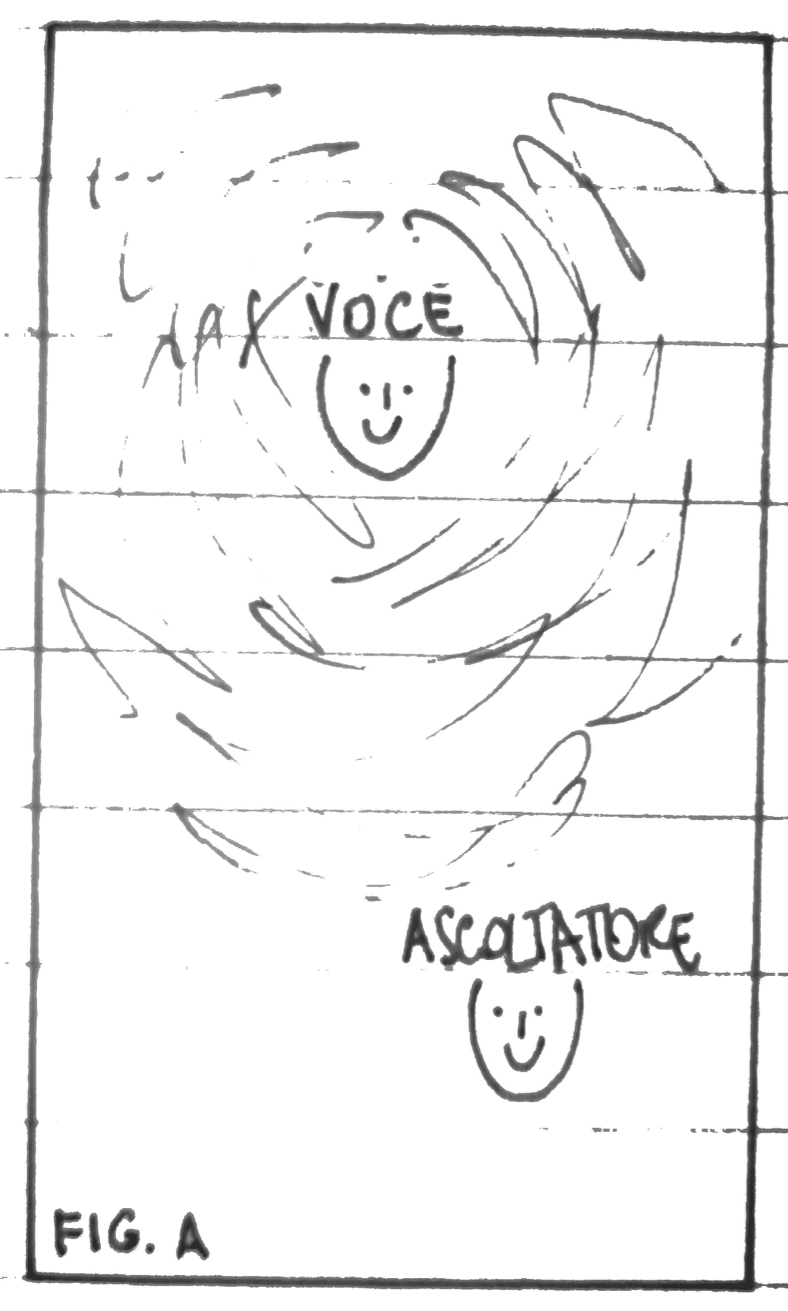
\includegraphics[width=.48\linewidth]{CAPITOLI/1000/IMG/figa.png}
%\caption{}
\label{ee:figa}
\end{center}
\end{figure}

Una voce nello spazio di una stanzetta si dirige, con una sua direzione, verso
un punto e contemporaneamente, con meno direzionalità, lateralemente, raggiunge
il resto della stanza. Questo meccanismo ha a che fare con la forma sonora di una
voce, prima ancora che con la forma architettonica della piccola stanza.

Dobbiamo immaginare la forma sonora come un'armatura attorno al nostro oggetto
sonoro, un'armatura fatta di fittissime molecole in vibrazione. Ogni suono ha una
sua veste plastica. Se vi dicessi ottavino e poi contrabbasso voi avreste già
collegato tutto ciò che vi serve per vederli, sentirli, ed ora, volendo, vestirli
della loro forma sonora. Ma cosa accade alla forma sonora di uno strumento in
presenza di tecninche estese applicate allo strumento? Una mano che inizia a produrre
suono li, nello stesso luogo dello strumento, a dove pochi minuti prima premeva
solo tasti (la mano  sinistra di UR) diventa esplosione di forma acustica e musicale.

Ecco questo è un po' il cuore di quello che vorrei fosse il mio dottorato di
ricerca che non avrò mai e un po' anche la manifestazionne di una piuttosto
triste verità: esclusi i percorsi individuali e rari percorsi di ricerca
non istituzionalizzata, la musica contemporanea ha esaurito la sua carica
contributiva al conoscimento, alla comprensione generalizzata.

Tornando alla forma, Questa si staglia nello spazio circostante e si espande e si muove
all'interno di questo spazio e ne viene modellata come una massa morbida all'interno
di un contenitore. Qui iniziano i fenomeni di riflessione e la forma si
cristallizza assumendo caratteristiche in funzione dello spazio e, quindi, del tempo.
L'ascoltatore che partecipa a questo evento vede una persona solida parlare nello
spazio di una stanza e sente la forma solida della voce provenire dalla sua bocca
e contemporaneamente, quindi subito dopo, dalla stanza sotto forma di riflessioni.
Sì! converremo infine, questa esperienza di ascolto rispetta queste qualità.

\begin{figure}[h]
\begin{center}
  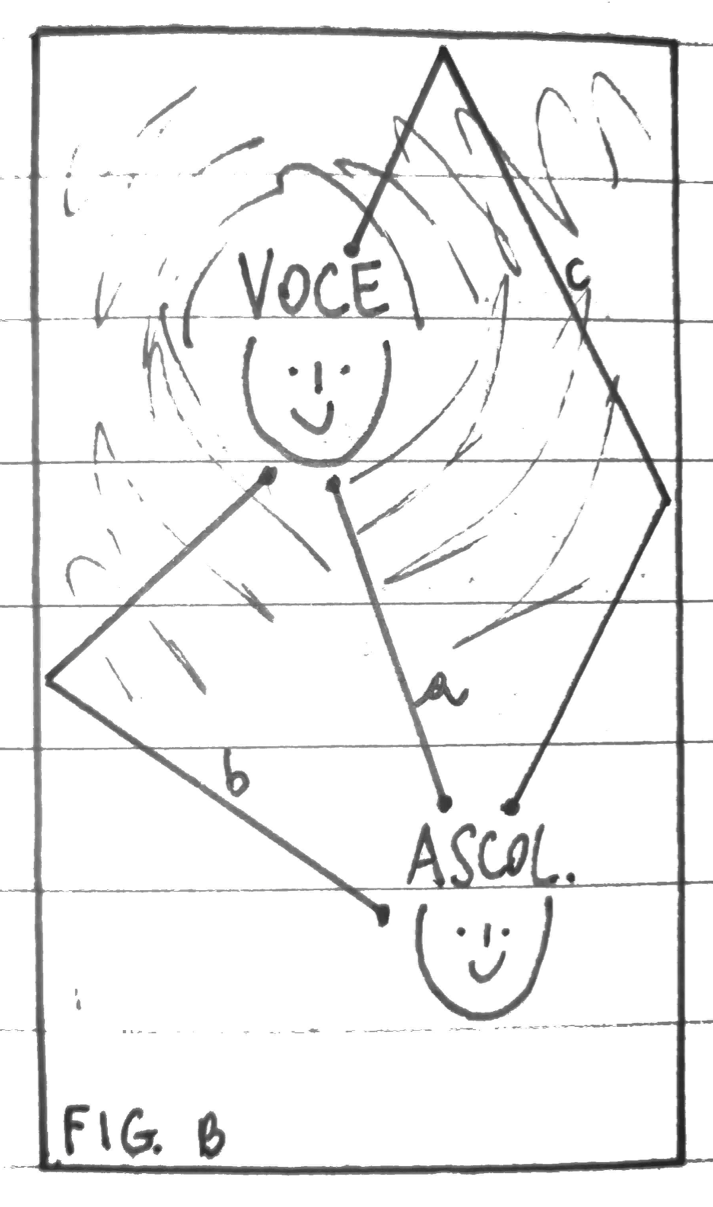
\includegraphics[width=.48\linewidth]{CAPITOLI/1000/IMG/figb.png}
%\caption{}
\label{ee:figb}
\end{center}
\end{figure}

Una voce che attraverso la sua forma acustica riempia uno spazio acustico è
un'esperienza d'ascolto stereofonica. Non è ancora giunto il momento di
interrompere la discussione dicendo: “ma come, non servono due diffusori?” Non
ancora, il problema è più complesso. È importante sottolineare che la stereofonia,
l'ascolto stereofonico, è una qualità dell'ascolto che si può osservare in
determinate circostanze e che richiede necessariamente il lavoro concertato delle
due orecchie. Un ascolto stereofonico è quindi possibile solo in coincidenza
con un ascolto \emph{binaurale}, ovvero effettuato con entrambe le orecchie.

Di nuovo una qualità che presuppone dei contenuti coerenti con delle
caratteristiche specifiche. Ora, nel mondo elettroacustico, del suono prodotto
o riprodotto elettricamente, dovremmo essere in grado di effettuare lo stesso
ragionamento sostituendo alla persona che parla un diffusore generico. Come per
l'essere umano, la voce è esempio di suono proprietario anche per il diffusore
si può scegliere un suono che lo caratterizzi elettroacusticamente, un suono
che lo rende particolare: il suono definito rumore rosa. Posizionato il diffusore
nella stessa stanza e con le stesse circostanze di ascolto precedenti, avremmo
una condizione di ascolto stereofonico? Ovviamente si. Un solo diffusore può
costituire una condizione d'ascolto stereofonica. In questo caso l'oggetto
acustico è un diffusore che esprime se stesso attraverso un suono non informativo.
Un rumore è caratterizzato da un'assenza di informazione, fatta esclusione del
fatto stesso che è rumore.

\begin{figure}[h]
\begin{center}
  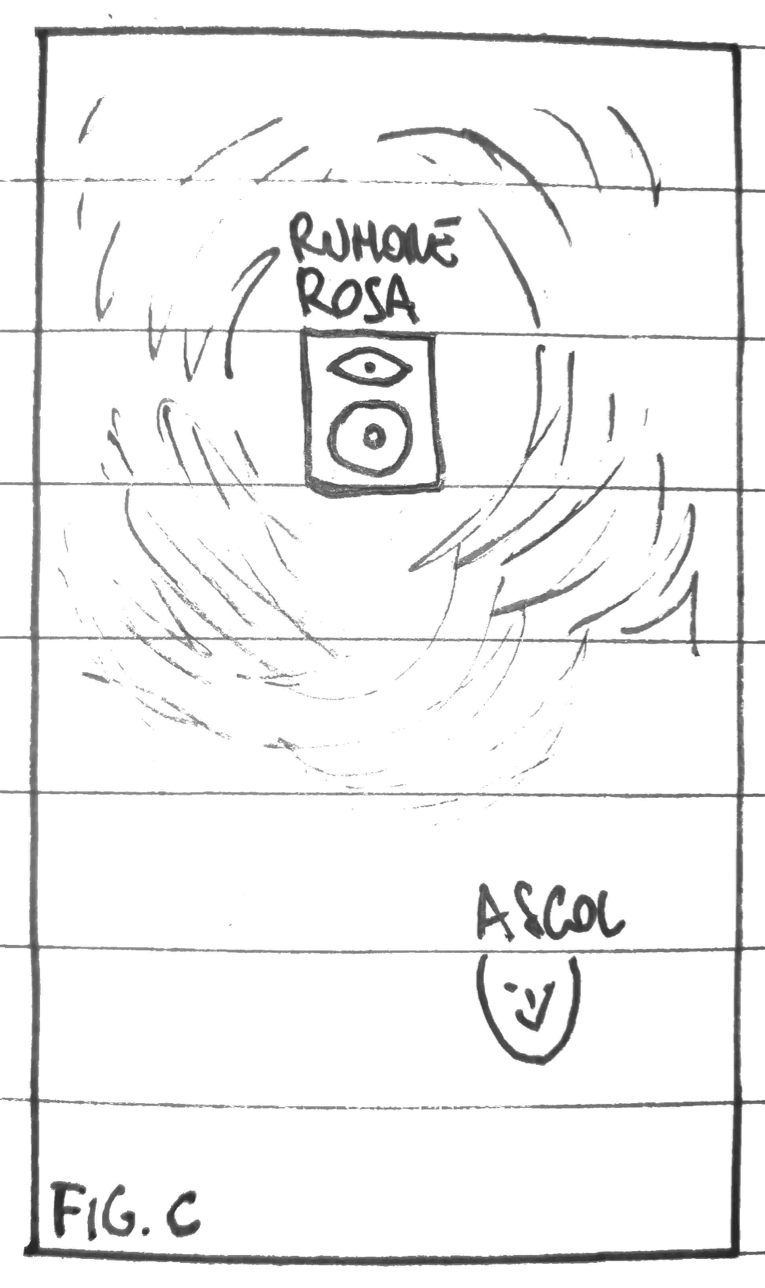
\includegraphics[width=.48\linewidth]{CAPITOLI/1000/IMG/figc.png}
%\caption{}
\label{ee:figc}
\end{center}
\end{figure}

che informazioni? be quelle che descrivono un suono come la percezione di altezza,
durata, intensità e timbro. Questa descirizione di stereofonia possibile anche
con un solo soggetto sonoro, voce o diffusore che sia, non è così comune e
condivisa. Ciò accade a causa del fatto che spesso si fa confusione tra stereofonia,
o stereofonica, come aggettivo applicato alla tecnica di diffusione e registrazione
piuttosto che alla qualità percettiva che queste tecniche dovrebbero suggerire.

Per arrivare a descrivere la tecnica dobbiamo percorrere ancora alcuni passi.

Nel momento in cui si passa da un dominio puramente acustico sia esso derivante
da una voce umana quanto un rumore diffuso attraverso un altoparlante, ad un
dominio di riproduzione acustica, ovvero di rappresentazione attraverso meccanismi
e tecniche allora cambia completamente lo scenario acustico e le circostanze di
ascolto. Un diffusore tradizionale può riprodurre una voce umana o un diffusore
che suona rumore rosa? Si certo che può riprodurli. Questa riproduzione
costituirebbe un ascolto stereofonico della sorgente originale? No, non lo sarebbe.

\begin{figure}[h]
\begin{center}
  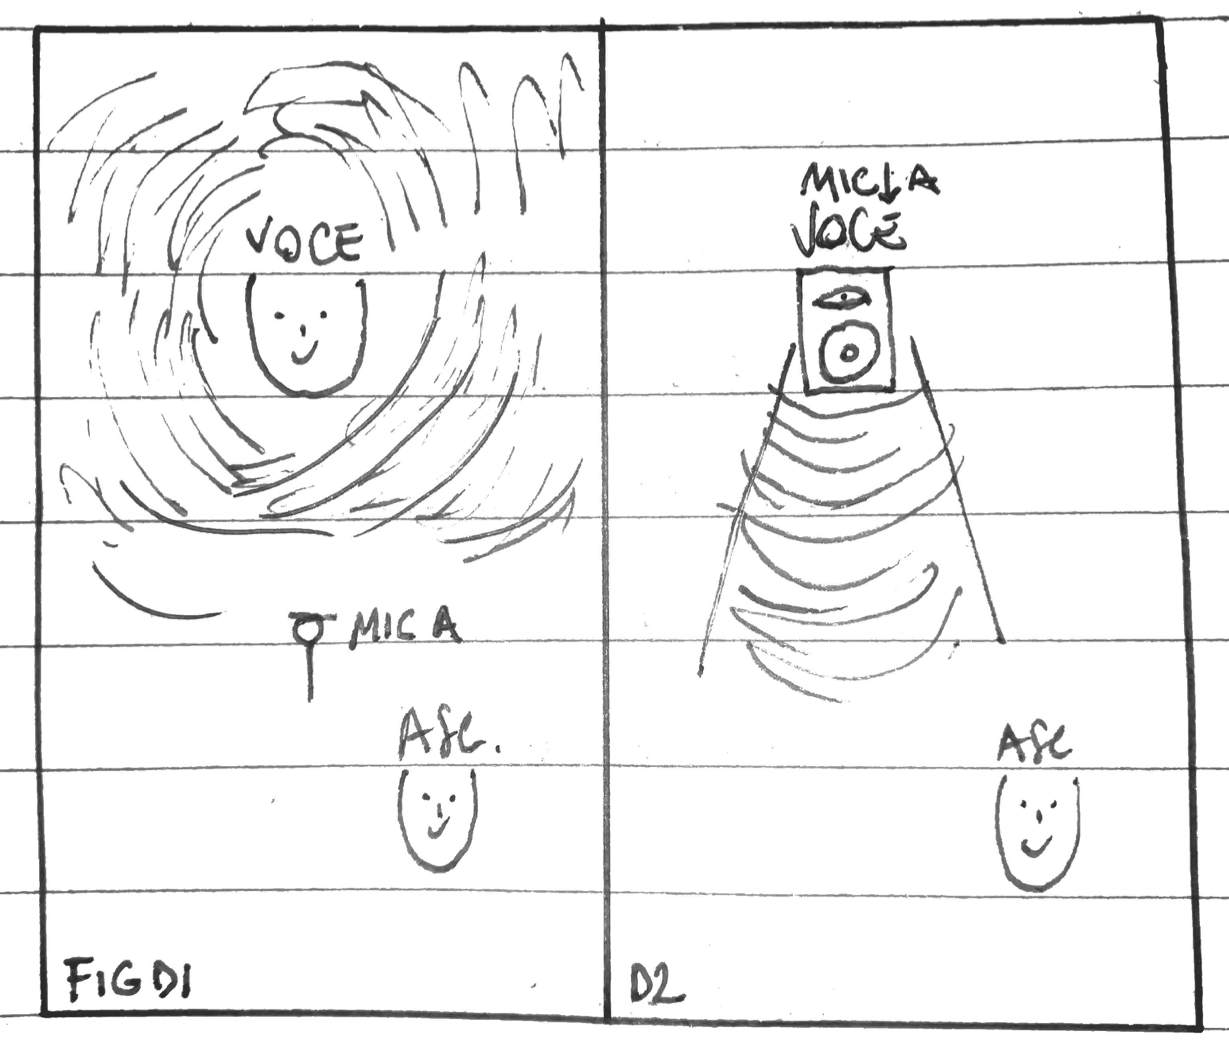
\includegraphics[width=.98\linewidth]{CAPITOLI/1000/IMG/figd1d2.png}
%\caption{}
\label{ee:figd1d2}
\end{center}
\end{figure}


\begin{quote}
When the music is reproduced through a single channel the echoes arrive from the same direction as the direct sound so that confusion result\footnote{Quando la musica viene riprodotta attraverso un singolo canale, gli echi arrivano dalla stessa direzione del suono diretto in modo tale da creare confusione.}.
\end{quote}

Qui si sviluppa tutta la questione, un solo diffusore non è in grado di rappresentare
la solidità originaria, la forma sonora dell'oggetto acustico originario, il suo
rapporto con lo spazio che lo ha modellato. Per comprendere meglio ogni possibile
questione legata alla diffusione sonora, mediante dispositivi elettroacustici ci
vorrebbe un minimo di tempo speso nella sperimentazione con lo strumento altoparlante.
Perché di questo si parla, di uno strumento tecnico, tecnologico, musicale e
profesisonale.

\begin{quote}
Ci sono problemi che alle volte anch'io non capisco, nel senso che se ne porgono
continuamnte di nuovi. È da anni che lavoro e sperimento negli studi di live electronics di
Friburgo, della Sudwestfunk. Si tratta delle trasformazioni in tempo reale del
suono e della voce, e del comporla con lo spazio, usando le tecnologie di oggi,
con i vari altoparlanti disposti nella sala. C'è qualcosa di nuovo solo sul piano
tecnico, perché  se prendiamo la Scuola di S. Marco veneziana di Andrea e Giovanni
Gabrieli, Monteverdi, di Willaert, con le composizioni a più cori, la grande
scuola spagnola all'epoca di Filippo II [\ldots] si faceva musica per otto organi
e quattro cori, cioè si suonava lo spazio come componente musicale, non come poi
la prassi dell'ottocento usa lo spazio, mettendo dentro l'orchestra e quel che
succede succede. Quindi altri studi, anche studi di fisica architettonica, studi
di processi di eco, di riverberazione, di materiali acustici. [\ldots] Qui una
composizione non è  data una volta per sempre, perché per ogni spazio noi dobbiamo
cambiare i programmi dei computer e modificando i rapporti della trasformazione si modifica anche il rapporto acustico; [\ldots] il grande fascino di questo per me
è veramente la non ripetitività. [\ldots] Un interprete non deve studiarsi la
parte ma veramente partecipare. [\ldots] Cioè vedi come noi possiamo con la
tecnologia di oggi studiare molto meglio, cioè studiare in un altro modo. \\
Luigi Nono 1986
\end{quote}

La parabola bacchiana si conclude con una nota autobiografica. Noi, che abbiamo
osservato da vicino la maledizione di Bacco, non possiamo più tacere e seminiamo,
il vento muoverà le orecchie penzolanti e porterà le nostre confessioni altrove.
%%%%%%%%%%%%%%%%%%%%%%%%%%%%%%%%%%%%%%%%%%%%%%%%%%%%%%%%%%%%%%%%%%%%%%%%%%%%%%%%%%%%%%%%%%%%%%%%%% fiune dalle esposizioni

Una singola voce umana, monofonica, sta parlando all'interno di una piccola
stanza, una condizione stereofonica accettabile? In accordo con Blumlein,
Sì! Questo è il primo punto fermo.

Michael Gerzon, dagli anni settanta agli anni novanta, dalle radici dell'era di
Blumlein ha saltato la linea con una dozzina di descrizioni chiare sulla
percezione e tentativi di progettare tecnologie di riproduzione per colmare il
divario rispetto al regno acustico.

\begin{quotation}
The ears and brain localize sounds according to many different mechanism. Among
the most important cues used are low frequency interaural phase (applicable up
to around 2\emph{KHz}, but dominant below 700\emph{Hz}) and localization by
amplitude differences between the two ears, predominantly above about
1\emph{KHz}. While other cues are also important, we have found that satisfying
both these cues, and making them mutually consistent for central listener facing
in any direction, leads to particularly robust and reliable localization
quality.\cite{mg92pdmsss}
\end{quotation}

%%%%%%%%%%%%%%%%%%%%%%%%%%%%%%%%%%%%%%%%%%%%%%%%%%%%%%%%%%%%%%%%%%%% SUBSECTION
%%%%%%%%%%%%%%%%%%%%%%%%%%%%%%%%%%%%%%%%%%%%%%%%%%%%%%%%%%%%%%%%%%%%%%%%%%%%%%%%
\subsection{Sul concetto di \emph{PanPot}}
\label{sec:panpot}

L'oggetto \emph{panner} è rappresentato da un potenziometro di controllo
(hardware o software, in entrambi i casi a controllo analogico o digitale) che
regola la distribuzione di un segnale su più canali componenti un campo sonoro
stereo o multicanale. Ogni mixer ha un \emph{panpot} (abbreviazione di
\emph{potenziometro di panoramica}), per ciascun canale sorgente in ingresso,
che regola l'azione del \emph{panner}.

%L'ultima precisazione riguarda il movimento panoramico. La distribuzione dell'energia
%o la condizione della coppia di segnali che regola il movimento panoramico troppo
%spesso sono descritti come la possibilità di muovere gli oggetti attorno alla posizione
%dell'ascoltatore.

Generalmente il \emph{panpot} viene descritto come un pomello che permette di
muovere i suoni tra la sinistra e la destra del panorama di diffusione, il che è
parzialmente vero e potenzialmente pericoloso in termini di immaginazione
acustica.

Soffermandosi ad analizzare il fenomeno acustico di un suono prodotto da un
oggetto in movimento tra la destra e la sinistra di un campo percettivo emergono
diversi problemi.

Il primo riguarda l'\emph{effetto doppler}. Siamo seduti su una panchina al
margine di una strada che si estende infinita agli estremi della nostra vista
periferica. Un mezzo di soccorso, con la sirena accesa, si avvicina percorrendo
la strada davanti al nostro viso, da sinistra verso destra: percepiamo
una variazione in frequenza al passaggio della sirena, in funzione della
velocità. L'\emph{effetto doppler} ci descrive come nel percorso di
avvicinamento a noi la frequenza sale lentamente fino al massimo ottenuto nel
momento in cui ci raggiunge per poi diminuire rapidamente in coincidenza con
l'allontanamento.

Ora siamo dei \emph{sound designer}, siamo seduti di fronte alla nostra console
analogica e dobbiamo replicare l'effetto sopra descritto. Applicando un
movimento da sinistra a destra, azionando il \emph{panpot} su un suono di sirena
statico, registrato fermo ad un metro di distanza, pur ruotando velocemente il
potenziometro non otteniamo variazioni in frequenza. Il suono si muove tra la
sinistra e la destra del sistema d'ascolto senza produrre il movimento nello
spazio ma solamente lo spostamento della posizione relativa al nostro punto di
ascolto. Ne deriva una prima conslusione: il \emph{panpot} regola una posizione
relativa, non stabilisce criteri di movimento.

Un altro problema emergente del pensare il \emph{panning} come un movimento
scaturisce dalla relazione della sorgente con l'ambiente circostante. Che
movimento può esserci senza tenere conto del luogo in cui la sorgente sonora si
trova? Un avvocato pronuncia la sua arringa in tribunale parlando ad alta voce,
camminando, rimbalzando tra destra e sinistra. La voce si propaga nello spazio
ed è inevitabile che se ne percepisca la variazione topologica, morfologica in
relazione con le caratteristiche architettoniche: a sinistra della stanza c'è
una parete di finestre, a destra un muro in cemento. Pur non avendo velocità
sufficiente ad innescare l'effetto doppler, la sua continua variazione di
posizione corrisponde ad una continua variazione di rapporto con l'ambiente che
lo circonda, in relazione ad ogni infinto punto di ascolto all'interno della
stanza. In altre parole, quel movimento assume significati diversi relativi al
punto di ascolto.

Dovendo simulare lo stesso effetto mediante l'azione sul panpot, otterremmo la
variazione di posizione della voce nello spazio, ma non la sua relazione con lo
spazio.

\begin{figure*}[t!]
    \centering
    \begin{subfigure}[t]{0.45\textwidth}
        \centering
        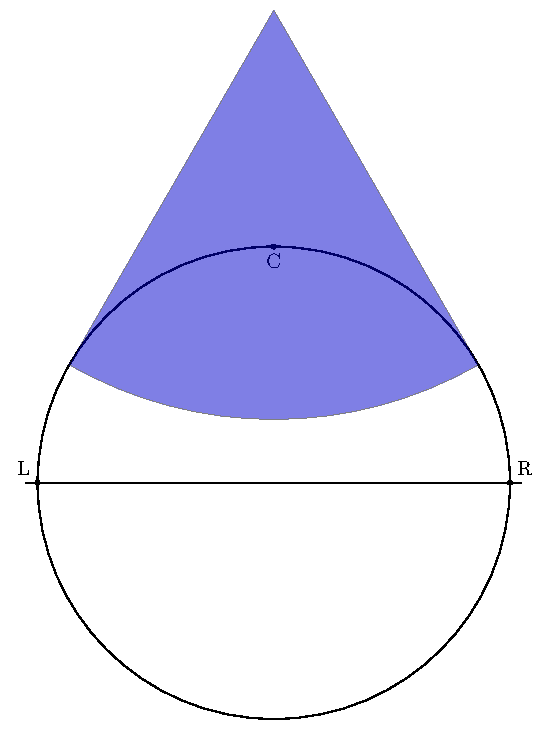
\includegraphics[height=8cm]{CAPITOLI/_TIKZ/PANNING/pan-frontal}
        \caption{Sorgente con incidenza frontale.}
        \label{pan:frontal}
    \end{subfigure}%
    ~
    \begin{subfigure}[t]{0.45\textwidth}
        \centering
        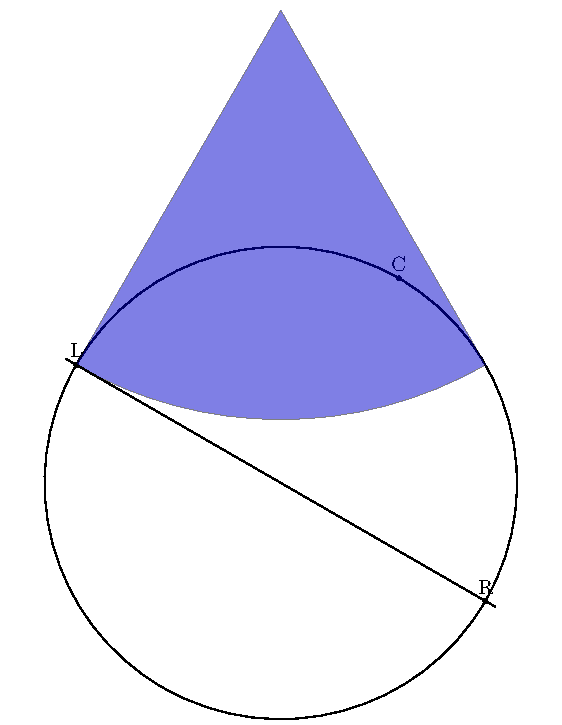
\includegraphics[height=8cm]{CAPITOLI/_TIKZ/PANNING/pan-left}
        \caption{Sorgente con incidenza laterale sinistra di 30 gradi.}
        \label{pan:left}
    \end{subfigure}
    \\
    \begin{subfigure}[t]{0.9\textwidth}
        \centering
        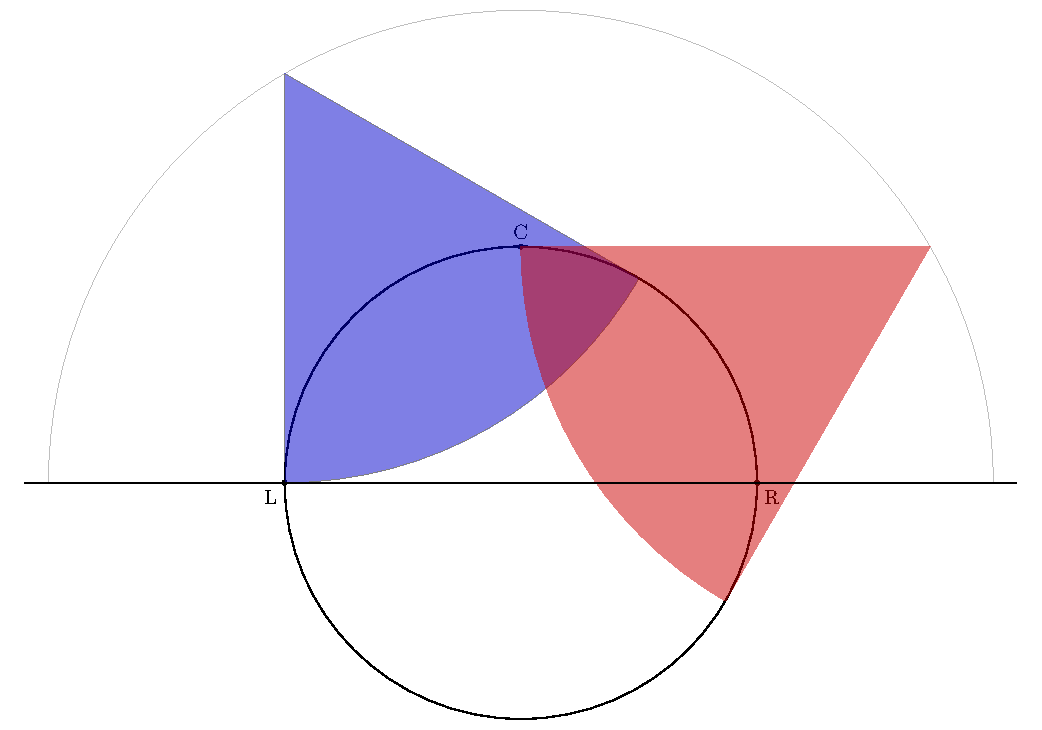
\includegraphics[height=8cm]{CAPITOLI/_TIKZ/PANNING/pan-both}
        \caption{Due sorgenti, una con incidenza laterale sinistra di 30 gradi,
        l'altra con incidenza laterale destra di 60 gradi.}
        \label{pan:both}
    \end{subfigure}
    \caption{La rotazione del \emph{PanPot} esegue una modifica della condizione
    di ascolto dell'ascoltatore, non un movimento della sorgente. Posizionando
    le singole sorgenti ci si pone in ascolto laterale, ruotati. Nella
    sovrapposizione di molteplici sorgenti il panorama risulta composto da
    ognuna di queste, con posizioni assolute ed angoli di incidenza relativi
    della testa.}
    \label{pan:all}
\end{figure*}

Il \emph{panpot}, nella sua capacità di descrizione della relazione tra i canali
che ricevono i suoi segnali, non muove la sorgente nello spazio, ma regola la
posizione della sorgente stessa in relazione al nostro punto di ascolto. In
altri termini il \emph{panner} non regola il movimento della sorgente, ma la
rotazione della testa in relazione ad essa. Il \emph{panner}, muove langolo di
incidenza del suono, ruota la testa, nei confronti della sorgente immobile.

Ogni \emph{panner} ha un'architettura interna che determina la quantità e la
condizione del segnale sorgente per ogni canale di destinazione. I più semplici
suddividono i segnali audio nei due canali sinistro e destro, attraverso un
opportuno controllo di guadagno (volume) discreto. La distribuzione dell'energia
tra i due canali è chiamata legge ed è descrivibile con una funzione matematica.

Come descritto da Blumlein, la sola variazione di ampiezza nella
rappresentazione del panorama stereofonico rappresenta una parte nella complessa
soddisfazione della percezione binaurale, non disegna l'intero meccanismo.
Per questo motivo, prima di descrivere i sistemi di panning di ampiezza, che
sono universalmente implementati su tutti i mixer del pianeta, è più opportuno
riprendere da dove egli stesso è partito. La visione di Blumlein fu ripresa in
seguito da Michael Gerzon, negli anni settanta, per sviluppare la tecnologia
\emph{ambisonic}, la quale rimane un atto di descrizione del mondo sonoro
percepito e riprodotto, nell'evoluzione della stereofonia, completamente diverso
da quello che commercialmente si è diffuso ed imposto.

%%%%%%%%%%%%%%%%%%%%%%%%%%%%%%%%%%%%%%%%%%%%%%%%%%%%%%%%%%%%%%%%%%%% SUBSECTION
%%%%%%%%%%%%%%%%%%%%%%%%%%%%%%%%%%%%%%%%%%%%%%%%%%%%%%%%%%%%%%%%%%%%%%%%%%%%%%%%
\subsection{Sul concetto di \emph{Diagramma Polare}}
\label{sec:polarplot}

Il diagramma polare (o curva polare) è invece un grafico a disegno circolare
dove i parametri sono dati dall’ampiezza e dall’angolo d’incidenza, mentre le
frequenze sono rappresentate da famiglie di curve. In presenza di un’unica curva,
si intende che questa è riferita ad una frequenza di $1KHz$. %piero

Un singolo segnale, nella sua oscillazione, espressa nella variazione di ampiezza
attorno allo zero, potrebbe essere derivato da qualsiasi tipo di microfono senza
un significato particolare. Potrebbe essere generato elettricamente da un
microfono con modello polare particolare o da una fonte sintetica senza
alcuna rilevanza specifica. La provenienza polare, la forma che assume la fase
del segnale, diventa rilevante nel confronto tra segnali.

Il diagramma polare di un microfono che, per caratteristiche costruttive, non
percepisce variazioni di angolo di incidenza del segnale, quindi non-direzionale,
è definito comunemente come omnidirezionale, la sua equazione contiene solo
variazioni di ampiezza, derivate della variazione di pressione dell'aria

\begin{equation}
ndp = 1(x)
\label{eq:omni}
\end{equation}

\begin{figure}[h]
\centering
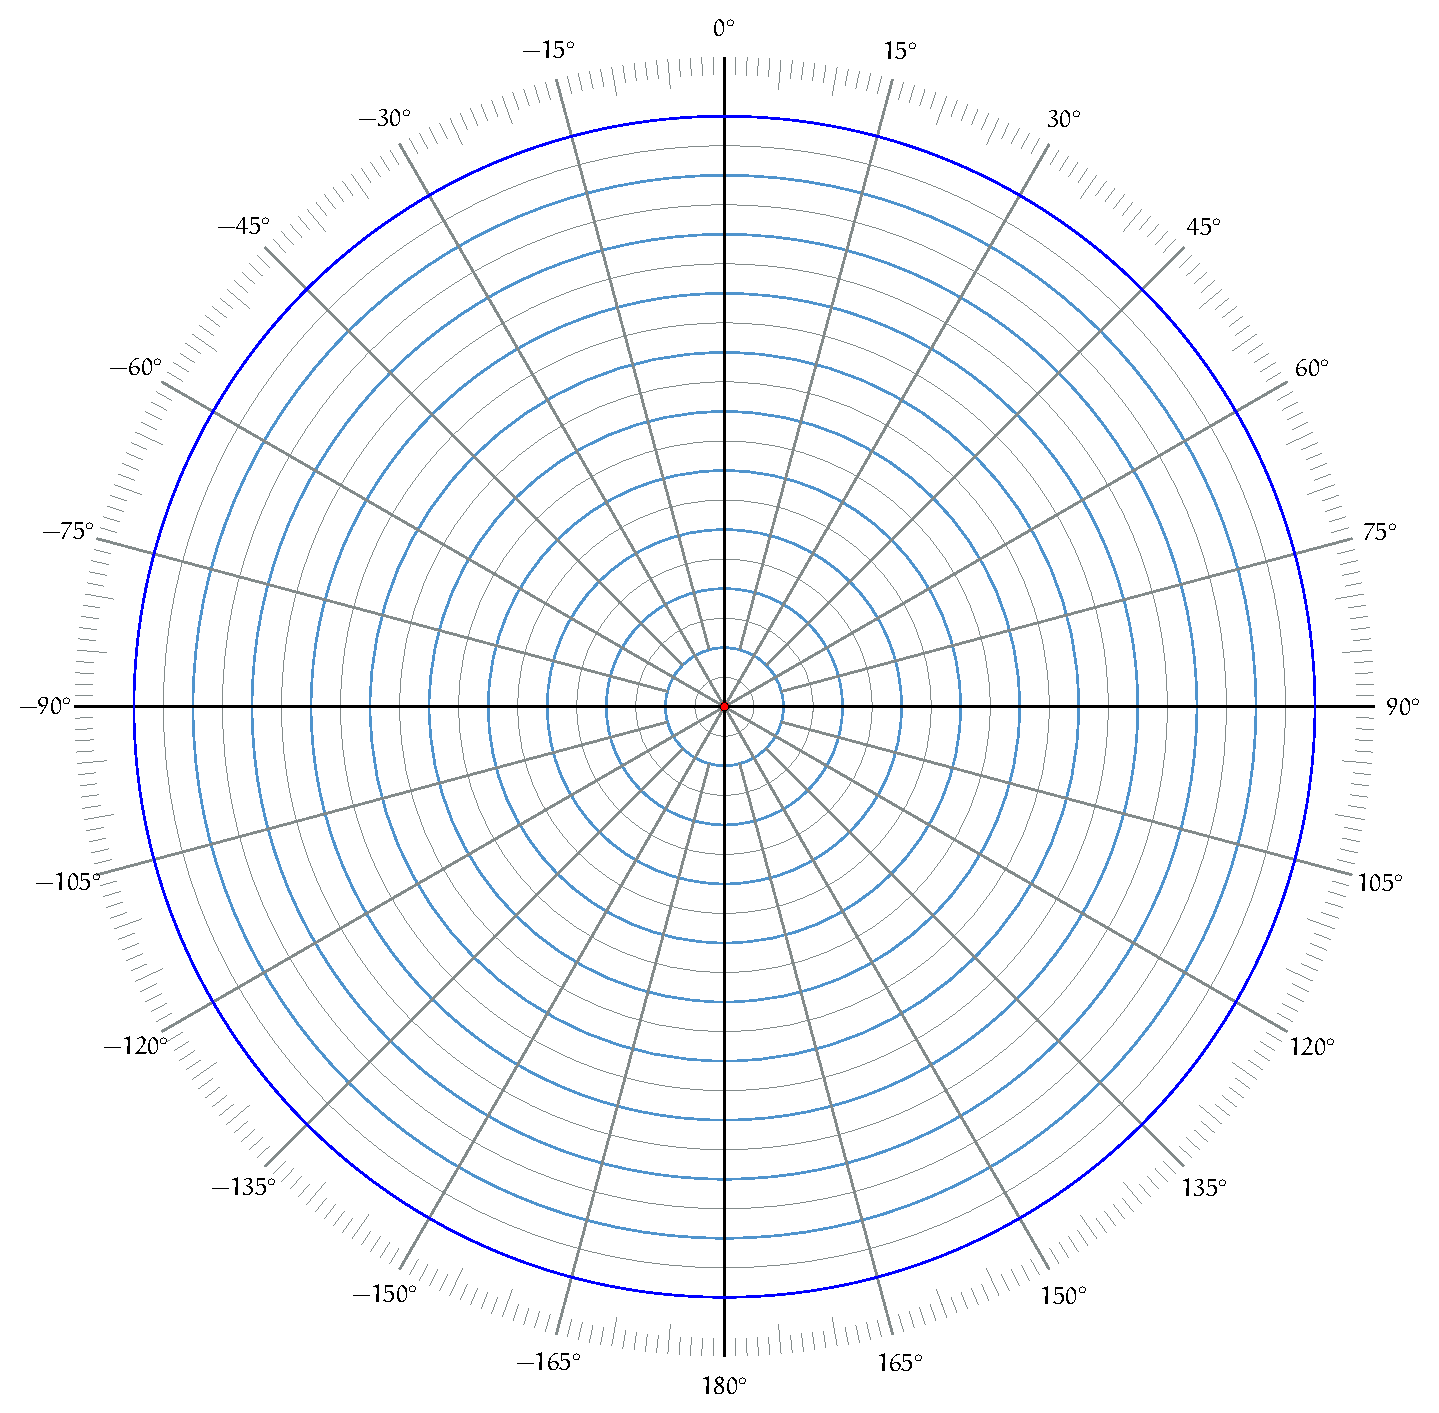
\includegraphics[width=1\columnwidth]{CAPITOLI/_TIKZ/POLAR/omni}
\caption{non-directional}
\label{polar:omni}
\end{figure}

%Il disegno nella parte sinistra di fig. 8 rappresenta la struttura di un tipico microfono a pressione (pressure microphone) omnidirezionale, mentre nella parte destra è rappresentata la sua curva polare, dove vediamo che la direzionalità del suono inizia ad essere percepita dal microfono a partire da circa 5 KHz in su, mentre le frequenze gravi non sono indicate in quanto assimilabili a quella rilevata a 1 KHz, cioè con attenuazione zero per qualsiasi angolo di provenienza del suono.
